\chapter{Introduction}


\begin{quote}
Drafting an introduction may feel like a daunting task. The writer must engage the audience in his or her research, provide the necessary background information about the topic, and set the stage for the study itself. How is this accomplished? First and foremost, there is no one formula. Consider the following: As under- graduates prepare to apply to graduate school they often ask faculty, ``What makes a successful application?'' The applicants invariably think in a formulaic fashion, believing that a secret formula exists - something akin to four parts research, two parts practical experience, GREs over a cutoff score, and an undergraduate GPA of at least 3.5. They believe that adherence to the recipe will fashion the ideal candidate. Sorry, there is no rigid formula. In fact, whereas the ingredients of the formula are indeed important to the evaluation process, different schools look differently at the varying credentials. \citep[][p. 41]{'4632'}
\end{quote}

Here, I introduce why I did what I did.
  
Figure~\ref{fig:Funnyhaha} helps to explain what happens if you mix math and children.

\begin{figure}[h!]
\centering
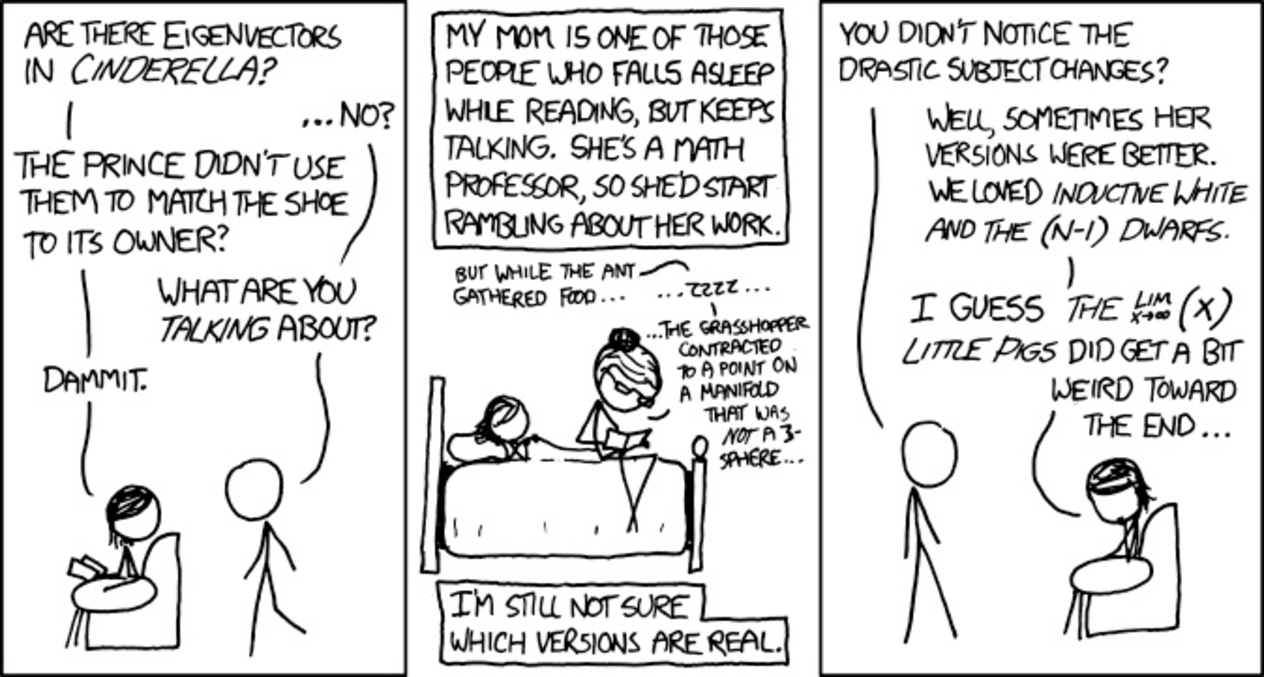
\includegraphics[width=0.7\textwidth]{figure/fairy_tales.pdf}
\caption{A funny caption used to lighten the mood while writing a dissertation.} \label{fig:Funnyhaha}
\end{figure}

Here is an example of a table in text with a footnote. You need to sure to reference Table \ref{tb:anova-pomega} prior to the table appearing the document. 

\begin{table}[ht!]
 \centering
 \begin{threeparttable}
 \caption{Summary of ANOVA by effect size estimates with partial-$\omega^2$}
 \label{tb:anova-pomega}
 \begin{tabular}{l C{.75in} C{.75in} C{.75in} C{.75in} C{.75in}}
   \toprule
 Effect & CFI & TLI & RMSEA & SRMRW & SRMRB\\ 
   \midrule
  $\rm N_1$            & 0.084 & 0.084 & 0.163 & 0.658 & 0.179 \\ 
 $\rm N_2$            & 0.028 & 0.029 & 0.023 & 0.666 & 0.581 \\ 
  $\mathrm{ICC}_O$  & 0.011 & 0.011 & 0.140 & 0.159 & 0.364 \\ 
  $\mathrm{ICC}_L$  & 0.010 & 0.010 & 0.008 & 0.042 & 0.138 \\ 
  Model           & 0.418 & 0.417 & 0.600 & 0.770 & 0.078 \\ 
  Estimator        & 0.051 & 0.051 & 0.261 & 0.449 & 0.191 \\ 
  $\rm N_1$:$\rm N_2$      & 0.076 & 0.076 & 0.060 & 0.281 & 0.023 \\ 
  $\rm N_1$:$\mathrm{ICC}_O$      & 0.010 & 0.011 & 0.005 & 0.000 & 0.140 \\ 
  $\rm N_1$:$\mathrm{ICC}_L$     & 0.001 & 0.001 & 0.009 & 0.005 & 0.043 \\ 
  $\rm N_1$:Model      & 0.002 & 0.002 & 0.010 & 0.113 & 0.002 \\ 
  $\rm N_1$:Estimator  & 0.004 & 0.004 & 0.004 & 0.015 & 0.000 \\ 
  $\rm N_2$:$\mathrm{ICC}_O$     & 0.003 & 0.003 & 0.020 & 0.010 & 0.018 \\ 
  $\rm N_2$:$\mathrm{ICC}_L$     & 0.012 & 0.012 & 0.005 & 0.007 & 0.058 \\ 
  $\rm N_2$:Model      & 0.007 & 0.007 & 0.043 & 0.097 & 0.005 \\ 
  $\rm N_2$:Estimator  & 0.072 & 0.072 & 0.149 & 0.074 & 0.010 \\ 
  $\mathrm{ICC}_O$:$\mathrm{ICC}_L$    & 0.007 & 0.007 & 0.008 & 0.001 & 0.117 \\ 
  $\mathrm{ICC}_O$:Model     & 0.016 & 0.016 & 0.062 & 0.006 & 0.023 \\ 
  $\mathrm{ICC}_O$:Estimator & 0.014 & 0.014 & 0.042 & 0.085 & 0.001 \\ 
  $\mathrm{ICC}_L$:Model     & 0.040 & 0.040 & 0.068 & 0.017 & 0.050 \\ 
  $\mathrm{ICC}_L$:Estimator & 0.029 & 0.029 & 0.002 & 0.108 & 0.008 \\ 
  Model:Estimator  & 0.043 & 0.043 & 0.065 & 0.026 & 0.004 \\
    \bottomrule
 \end{tabular}
 	\begin{tablenotes}[para,flushleft]
    {\small
        \textit{Note.} The meaning of each value can be interpreted as follows. For example, for the effect of level-1 sample size ($\rm N_1$), 8.4\% of the variability in observed CFI scores can be attributed to the number of level-1 units were sampled per group after controlling for all other design factors (i.e., $\rm N_2$, $\mathrm{ICC}_O$, $\mathrm{ICC}_L$, and bivariate interactions).
    }
 	\end{tablenotes}
 \end{threeparttable}
 \end{table}





